\documentclass[11pt]{article}
\usepackage[top=1cm, bottom=2cm, left=1cm, right=1cm]{geometry}
\usepackage{ctex}
\usepackage{float}
\usepackage{algorithm}
\usepackage{algorithmicx}
\usepackage{algpseudocode}
\usepackage{amsthm,amsmath,amssymb}
\usepackage[colorlinks=true,linkcolor=blue]{hyperref}
\usepackage{listings}
\usepackage{xcolor,xparse}
\usepackage{realboxes}
\usepackage{graphics}
\usepackage{graphicx}
\usepackage{mathrsfs}
\usepackage{wrapfig}
\usepackage{subfigure}
\usepackage{pifont}

\definecolor{cmdbg}{rgb}{0.9,0.9,0.9}
\lstset{%
	basicstyle=\ttfamily,
	breaklines = true,
	backgroundcolor=\color{cmdbg},
}
\DeclareDocumentCommand{\ccmd}{v}{% 参数 v 表示工作方法类似于 \verb
    \Colorbox{cmdbg}{\csname lstinline\endcsname!#1!}%
}

\makeatletter
\newenvironment{breakablealgorithm}
  {% \begin{breakablealgorithm}
   \begin{center}
     \refstepcounter{algorithm}% New algorithm
     \hrule height.8pt depth0pt \kern2pt% \@fs@pre for \@fs@ruled
     \renewcommand{\caption}[2][\relax]{% Make a new \caption
       {\raggedright\textbf{\ALG@name~\thealgorithm} ##2\par}%
       \ifx\relax##1\relax % #1 is \relax
         \addcontentsline{loa}{algorithm}{\protect\numberline{\thealgorithm}##2}%
       \else % #1 is not \relax
         \addcontentsline{loa}{algorithm}{\protect\numberline{\thealgorithm}##1}%
       \fi
       \kern2pt\hrule\kern2pt
     }
  }{% \end{breakablealgorithm}
     \kern2pt\hrule\relax% \@fs@post for \@fs@ruled
   \end{center}
  }
\makeatother

\author{李明钰 22307110156}
\title{计算物理作业8}

\begin{document}
\maketitle


\section{题目1:解Possion方程}
\subsection{题目描述}
Consider the Poisson equation$\nbla^2 \phi(x,y)=-\rho/\epsilon_0$from electrostatics on a rectangular geometry with $x \in [0,L_x]$ and $y \in [0,Ly]$ Write a program that solves this equation using the relaxation method. Test your program with:
\mathrm{(a)~}\rho(x,y)=0,\varphi(0,y)=\varphi(L_x,y)=\varphi(x,0)=0,\varphi(x,L_y)=1\mathrm{V,~}L_x=1\mathrm{m,and~}L_y=1.5\mathrm{m;}\\\mathrm{(b)~}\rho(x,y)/\varepsilon_0=1\mathrm{V/m}^2,\varphi(0,y)=\varphi(L_x,y)=\varphi(x,0)=\varphi(x,L_y)=0,\mathrm{and~}L_x=L_y=1\mathrm{m.}



\subsection{程序描述}
先将泊松方程的右边$\rho/\epsilon_0$视作一个整体的$f(x,y)$,然后和边界条件一起作为输入输入松弛算法(算法\ref{Relaxation Method for Poisson Equation})即可得到两个不同情况下的泊松方程的解。
\subsection{伪代码}
\begin{breakablealgorithm}
    
\caption{Relaxation Method for Poisson Equation}
\label{Relaxation Method for Poisson Equation}
\begin{algorithmic}[1]
\State \textbf{Input:} Function $f$ (Poisson equation right-hand side), Grid $Z$ (with boundary conditions)
\State \textbf{Output:} Solution grid $Z$
\State Set $n_x = \text{number of columns in } Z$
\State Set $n_y = \text{number of rows in } Z$
\For{inter = 1 \textbf{to} max\_inter}
    \State $Z_{\text{new}} \gets Z$
    \For{$i = 1$ \textbf{to} $n_y - 1$}
        \For{$j = 1$ \textbf{to} $n_x - 1$}
            \State $Z_{\text{new}}[i,j] \gets \frac{1}{4} \left( Z[i+1,j] + Z[i-1,j] + Z[i,j+1] + Z[i,j-1] - h^2 f[i,j] \right)$
        \EndFor
    \EndFor
    \State $err \gets \max \left( \left| Z_{\text{new}} - Z \right| \right)$
    \State $Z \gets Z_{\text{new}}$

\EndFor
\State \textbf{Return} $Z$
\end{algorithmic}
\end{breakablealgorithm}

\subsection{输入输出实例}
\begin{figure}[htbp]
	\centering
	\subfigure[三维视图] {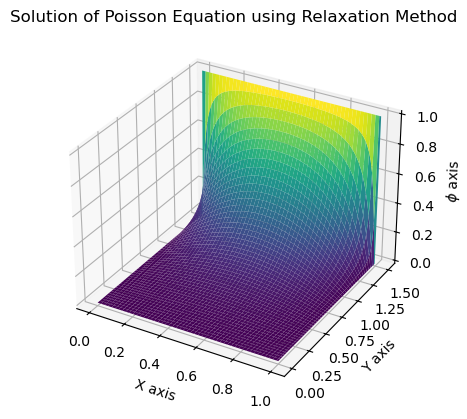
\includegraphics[width=.3\textwidth]{1.png}}
	\subfigure[二维视图] {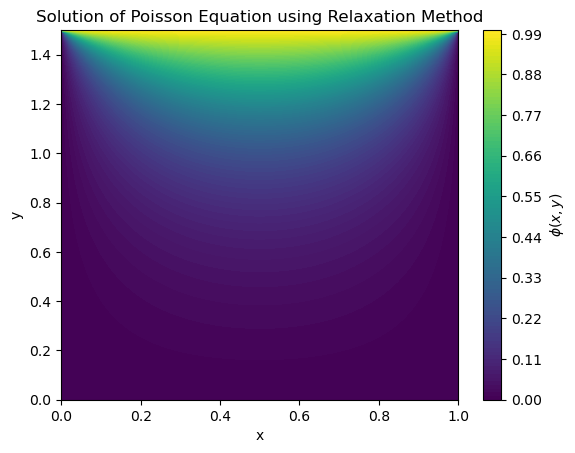
\includegraphics[width=.3\textwidth]{2.png}}
	\caption{用松弛法解第一问泊松方程}
	\label{fig:用松弛法解第一问泊松方程}
\end{figure}
\begin{figure}[htbp]
	\centering
	\subfigure[三维视图] {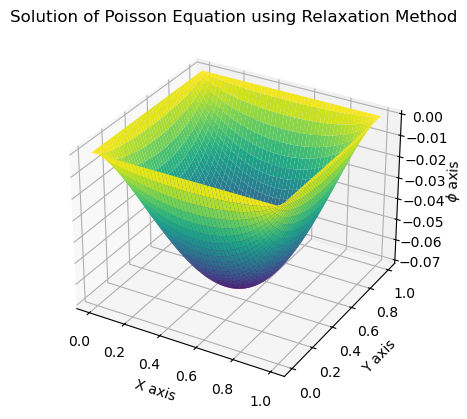
\includegraphics[width=.3\textwidth]{3.png}}
	\subfigure[二维视图] {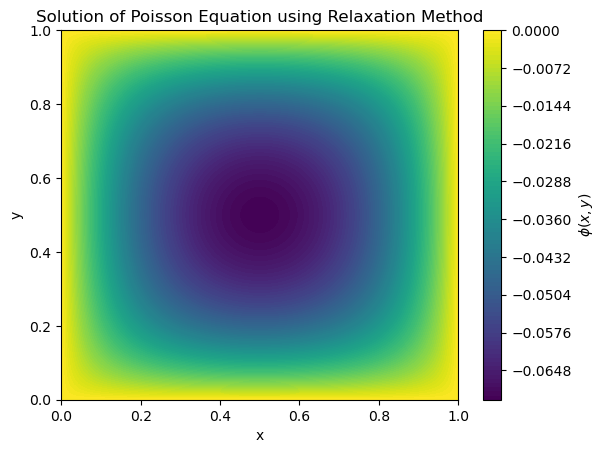
\includegraphics[width=.3\textwidth]{4.png}}
	\caption{用松弛法解第二问泊松方程}
	\label{fig:用松弛法解第二问泊松方程}
\end{figure}


\section{题目2:解含时薛定谔方程}
\subsection{题目描述}
Solve the time-dependent Schrodinger equation using both the Crank–Nicolson scheme and stable explicit scheme. Consider the one-dimensional case and test it by applying it to the problem of a square well with a Gaussian initial state coming in from the left.
\subsection{程序描述}
本程序使用自然单位制度,使用rank-Nicolson Scheme(算法\ref{Crank-Nicolson Scheme for Schrödinger Equation})和Explicit Scheme(算法\ref{Explicit Scheme for Schrödinger Equation})的数值计算方法解出了一维情况下质量$m=1$的粒子在方势阱:
\begin{equation}
    V(x) = \begin{cases}
    -V_0 = -1 & |x|<0.5 \\
    0 & other \quad cases
    \end{cases}
\end{equation}
下的含时薛定谔方程
\begin{equation}
    i\frac{\partial \Psi}{\partial t} = -\frac{1}{2m}\frac{\partial^2 \Psi}{\partial x^2} + V(x) \Psi 
\end{equation}
\subsection{伪代码}
\begin{breakablealgorithm}

\caption{Crank-Nicolson Scheme for Schrödinger Equation}
\label{Crank-Nicolson Scheme for Schrödinger Equation}
\begin{algorithmic}[1]
\State \textbf{Input:} Potential $V$, Initial wavefunction $\psi_0$
\State \textbf{Output:} Time-evolved wavefunction $\Psi$
\State Set $\Psi \gets \text{zeros}(Nt, Nx)$
\State Set $\Psi[0, :] \gets \psi_0$ \Comment{Initial wavefunction}
\State Set $\alpha \gets \frac{h_t}{h_x^2}$ \Comment{Discretization coefficient for Crank-Nicolson}
\State Set $B \gets \text{zeros}(Nx, Nx)$ \Comment{Matrix for discretized equation}
\For{a = 0 \textbf{to} $Nx - 1$}
    \For{b = 0 \textbf{to} $Nx - 1$}
        \If{$a - b = 0$}
            \State $B[a, b] \gets -0.5 V[a] \frac{h_t}{\hbar} - 0.5 \alpha \frac{\hbar}{m}$
        \ElsIf{$|a - b| = 1$}
            \State $B[a, b] \gets 0.25 \alpha \frac{\hbar}{m}$
        \EndIf
    \EndFor
\EndFor

\For{$j = 1$ \textbf{to} $Nt - 1$}
    \State $\Psi[j] \gets \left( i \cdot I_{Nx} + B \right)^{-1} \left( i \cdot I_{Nx} - B \right) \Psi[j - 1]$
\EndFor

\State \textbf{Return} $\Psi$
\end{algorithmic}
    
\end{breakablealgorithm}

\begin{breakablealgorithm}
    
\caption{Explicit Scheme for Schrödinger Equation}
\label{Explicit Scheme for Schrödinger Equation}
\begin{algorithmic}[1]
\State \textbf{Input:} Potential $V$, Initial wavefunction $\psi_0$
\State \textbf{Output:} Time-evolved wavefunction $\Psi$
\State Set $\alpha \gets \frac{h_t}{h_x^2}$ \Comment{Discretization coefficient}
\State Set $\Psi \gets \text{zeros}(Nt, Nx)$
\State Set $\Psi[0] \gets \psi_0$ \Comment{Initial wavefunction}
\State Set $A \gets \text{diagonal matrix with entries} \left( -i \frac{\hbar^2}{m} \alpha - i h_t V \right)$ \Comment{Matrix A}
\State Set $A \gets A + \text{off-diagonal elements} \left( i \frac{\hbar^2}{2m} \alpha \right)$
\State Set $\Psi[1] \gets \psi_0 + A \psi_0$
\For{$j = 2$ \textbf{to} $Nt - 1$}
    \State Set $A \gets \text{zeros}(Nx, Nx)$
    \For{$a = 0$ \textbf{to} $Nx - 1$}
        \For{$b = 0$ \textbf{to} $Nx - 1$}
            \If{$a - b = 0$}
                \State $A[a, b] \gets -2j \frac{\hbar^2}{m} \alpha - 2j h_t V[a]$
            \ElsIf{$|a - b| = 1$}
                \State $A[a, b] \gets i \frac{\hbar^2}{m} \alpha$
            \EndIf
        \EndFor
    \EndFor
    \State $\Psi[j] \gets \Psi[j-2] + A \Psi[j-1]$ \Comment{Explicit step for time evolution}

\EndFor
\State \textbf{Return} $\Psi$
\end{algorithmic}
\end{breakablealgorithm}

\subsection{输入输出实例}
结果如图\ref{fig:两种不同方法解含时薛定谔方程}所示,可以发现两种解法得到的解相差很小。
\begin{figure}[htbp]
	\centering
	\subfigure[Crank-Nicolson Scheme] {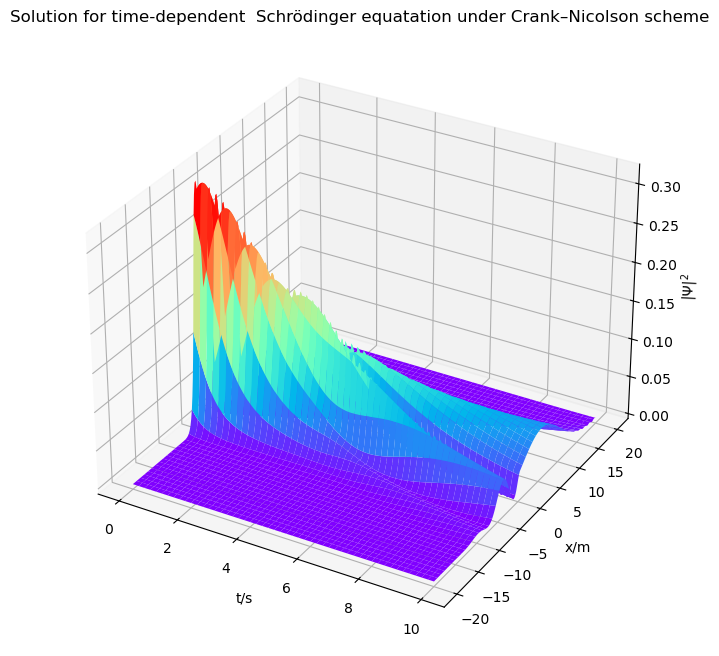
\includegraphics[width=.3\textwidth]{5.png}}
	\subfigure[Explicit Scheme] {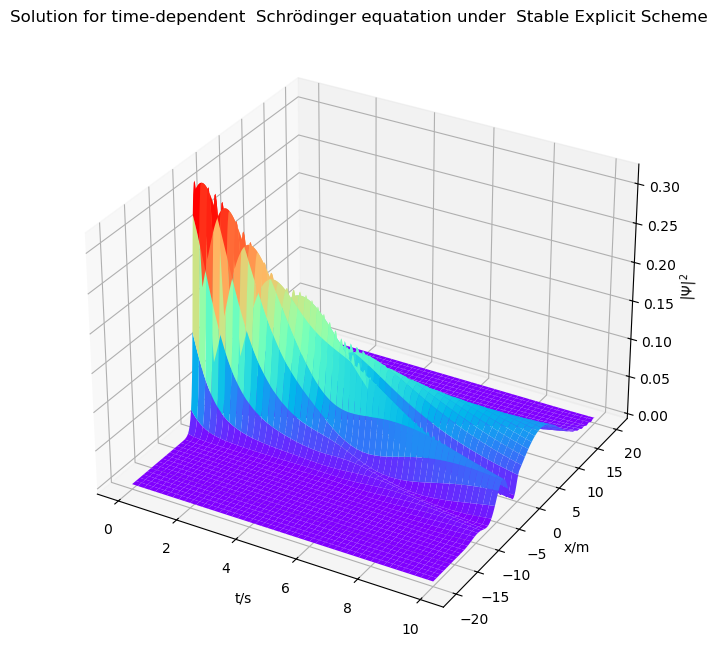
\includegraphics[width=.3\textwidth]{6.png}}
	\caption{两种不同方法解含时薛定谔方程}
	\label{fig:两种不同方法解含时薛定谔方程}
\end{figure}
\end{document}
